%(BEGIN_QUESTION)
% Copyright 2009, Tony R. Kuphaldt, released under the Creative Commons Attribution License (v 1.0)
% This means you may do almost anything with this work of mine, so long as you give me proper credit

Read and outline the ``Molecular Quantities'' section of the ``Chemistry'' chapter in your {\it Lessons In Industrial Instrumentation} textbook.  Note the page numbers where important illustrations, photographs, equations, tables, and other relevant details are found.  Prepare to thoughtfully discuss with your instructor and classmates the concepts and examples explored in this reading.

\underbar{file i04111}
%(END_QUESTION)




%(BEGIN_ANSWER)


%(END_ANSWER)





%(BEGIN_NOTES)

One ``mole'' of a substance is equal to 6.022 $\times 10^{23}$ molecules.  This is the quantity necessary for the mass of a 1-mole sample to be equal in grams to the molecular weight (sum of atomic masses) of the molecules comprising the sample.  In order to calculate the mass of a sample, take the molecular weight of the molecules comprising that sample (i.e. the sum total of all atomic masses for each of the constituent elements times the number of atoms for each of the elements in the molecule) and multiply that by the number of moles in the sample.

The molecular weight of a substance may be used as a unity fraction for converting sample mass to moles, or vice-versa.  For example, since we know the molecular weight of sodium chloride (NaCl = 23 + 35.5 = 58.5), we may express this as a unity fraction (58.5 grams per mole, or 1 mole per 58.5 grams) in any problem where we need to calculate the mass or molar quantity of a sodium chloride sample.

\vskip 10pt

The concentration of a solute in a liquid solution is often expressed as a {\it molarity}, which is the number of moles of solute dissolved in the total volume of liquid (liters), or mols/liter.

\vskip 10pt

Concentrations may also be specified as percent, ppm, or ppb.  These are merely ratios of solute to solution, either in volumetric terms or in mass terms.


\vskip 20pt \vbox{\hrule \hbox{\strut \vrule{} {\bf Suggestions for Socratic discussion} \vrule} \hrule}

\begin{itemize}
\item{} Demonstrate how the ``unity fraction'' method of unit conversions works well to convert between moles and mass units for any substance.
\item{} $6.022 \times 10^{23}$ seems like an awfully arbitrary quantity to use as the definition of a ``mole.''  Explain why this is {\it not} an arbitrary number.
\item{} Explain why one mole of oxygen atoms (O) does not possess the same mass as one mole of oxygen molecules (O$_{2}$), or the same mass as one mole of ozone molecules (O$_{3}$).
\item{} Calculate the mass of four moles of {\it ozone} gas (O$_{3}$) molecules.
\item{} Closely examine the label shown on the calibration gas bottle and describe some of the pertinent information presented on it.
\end{itemize}















\vfil \eject

\noindent
{\bf Prep Quiz:}

Calculate the mass (in grams) of exactly four moles of potassium (K) atoms:

$$\includegraphics[width=15.5cm]{i04111x01.eps}$$

\begin{itemize}
\item{} 156.4 grams
\vskip 5pt 
\item{} 76.00 grams
\vskip 5pt 
\item{} 80.00 grams
\vskip 5pt 
\item{} 39.09 grams
\vskip 5pt 
\item{} 43.09 grams
\vskip 5pt 
\item{} 9.773 grams














\vfil \eject

\noindent
{\bf Prep Quiz:}

Calculate the mass (in grams) of exactly three moles of potassium (K) atoms:

$$\includegraphics[width=15.5cm]{i04111x01.eps}$$

\begin{itemize}
\item{} 117.3 grams
\vskip 5pt 
\item{} 57.00 grams
\vskip 5pt 
\item{} 60.00 grams
\vskip 5pt 
\item{} 39.09 grams
\vskip 5pt 
\item{} 42.09 grams
\vskip 5pt 
\item{} 13.03 grams
\end{itemize}

%INDEX% Reading assignment: Lessons In Industrial Instrumentation, Chemistry (LEL and UEL explosive limits)

%(END_NOTES)


